\section{Medical Imaging Techniques}

    Medical Image Segmentation aims to determine the location and shape of the body part or structure within a 2D or 3D image automatically or semi-automatically \cite{merjulah2019classification}.
    The medical images are acquired using different modalities.
    Wide modality range and the high variability of human anatomy is the major difference of medical image segmentation.
    Medical images are divided into several interests related with the problem definition to detect or segment the tumor or mass.
    Irregularities, blurred vision borders, low contrast between lesion and skin, air bubles are the some of various artifacts that makes segmentation medical imaging challenging \cite{guo2019neutrosophic}.

    Medical Imaging Techniques (MIT) are concerned to create medical images to be able to examine internal structures of body without opening up it \cite{kasban2015comparative}.
    In this section, common medical imaging techniques are being investigated.

    \subsection{Common Diagnostic Modalities}

        \begin{figure}
    \centerline{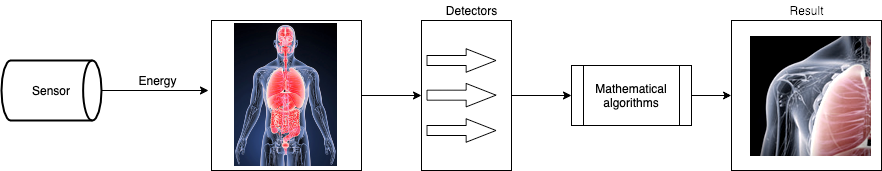
\includegraphics[width=1\columnwidth]{02-related-works/figures/medical-imaging-system-concept.png}}
    \caption{Medical Imaging Concept}
    \label{fig:medical-imaging-system-concept}
\end{figure}

        This section represent the review of widely-used medical imaging techniques namely X-ray Radiography,
        Magnetic Resonance Imaging, and Computed Tomography. The flowchart of a generic procedure in medical imaging
        is given in Figure ~\ref{figure:medical-imaging-system-concept}.

        \begin{itemize}

            \item \textbf{X-ray Radiography} is an imaging technique that uses ionizing electromagnet radiation, such as X-ray which is a type of high-energy electromagnetic radiation \cite{kasban2015comparative}.
                    As it can be seen in Figure~\ref{figure:sample-xray-images}, there is a trade-off between radiation level and image contrast which should be chosen carefully.
                    X-ray passes through the body and is absorbed at different levels according to several factors such as the different tissue density.
                    Mammography which deals with the scanning of breast tissue is one of the well-known application areas of X-ray Radiography.

                    \begin{figure}
    \centerline{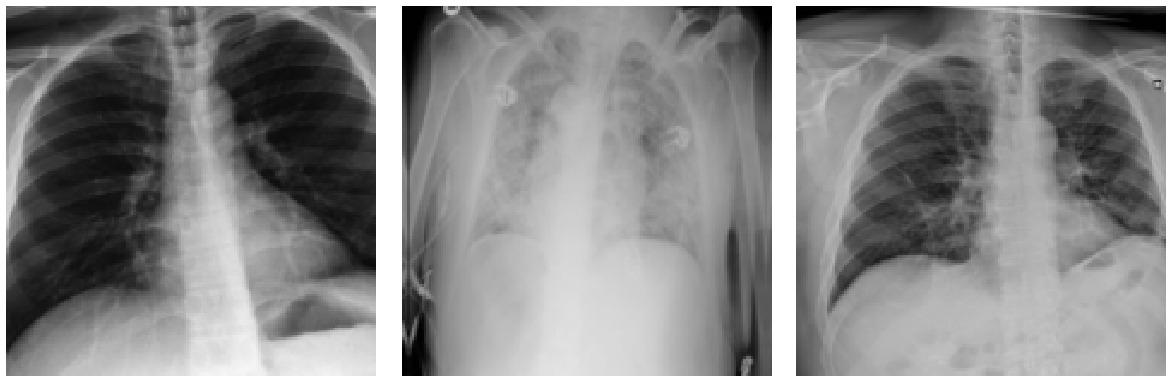
\includegraphics[width=1\columnwidth]{02-related-works/figures/sample-xray-images.png}}
    \caption{Sample X-ray Images \cite{ChestXRa12online}}
    \label{figure:sample-xray-images}
\end{figure}

            \item \textbf{Magnetic Resonance Imaging (MRI)} is a commonly used imaging techniques for medical tasks
                    which uses magnetic fields and frequencies in the radio wave spectrum to create images of body tissue \cite{mehmood2013prioritization}.
                    Magnetic spin relaxation times and proton density changes can be used as distinctive in detecting abnormal tissues.
                    MRI is based on visualizing these changes.
                    MRI imaging can be enhanced by using a contrast solution, e.g. gadolinium, which will change the relaxation properties of some tissues under certain conditions.

                    \begin{figure}
    \centerline{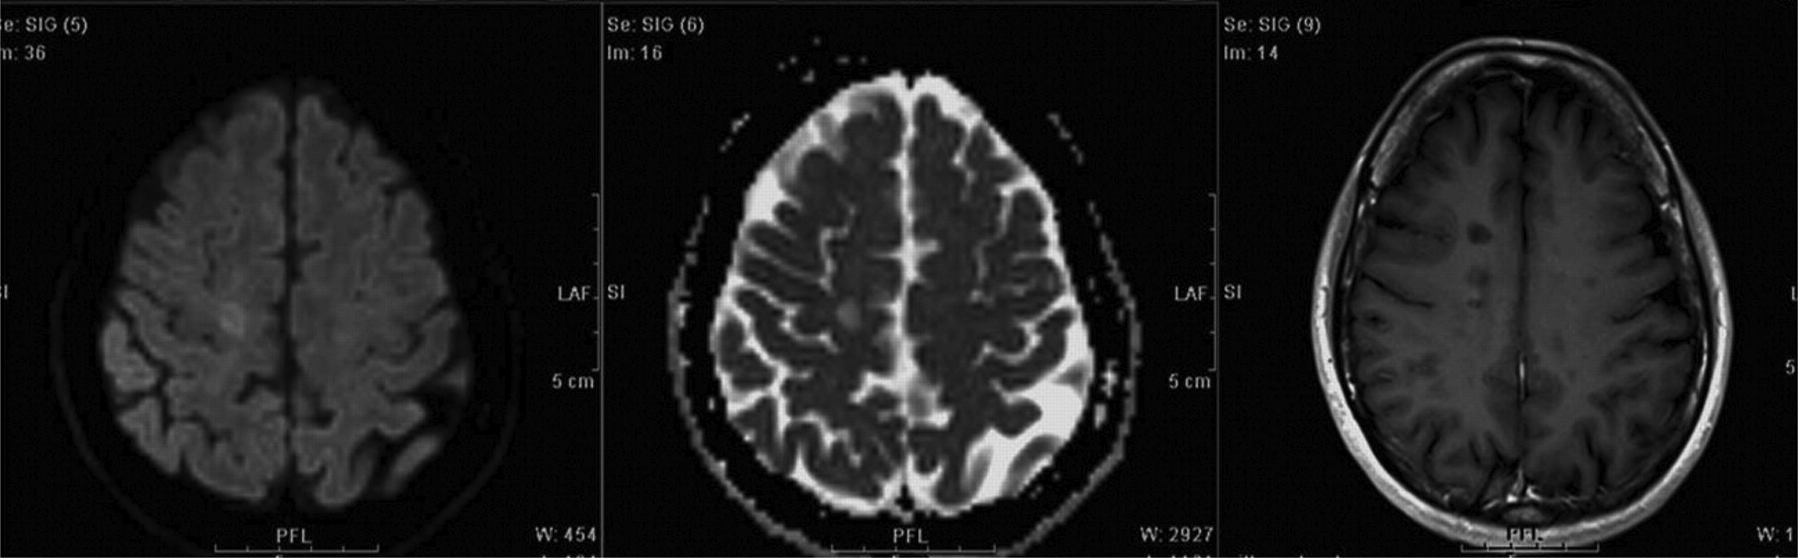
\includegraphics[width=1\columnwidth]{02-related-works/figures/sample-mri-images.png}}
    \caption{Sample MRI Images \cite{lovblad2010mr}}
    \label{figure:sample-mri-images}
\end{figure}

                    Advantages of using MRI include painless, ionizing-free radiation, and high spatial resolution with operator independent usage.
                    MRI does not offer real time results because of the relatively long scanning and post processing time.
                    Moreover, patient comfort is an issue due to limited space within the gantry and long acquisition time.
                    An MRI sample is shown in Figure~\ref{figure:sample-mri-images}.

            \item \textbf{Computed Tomography (CT)} is supported with a cathode ray tube used to create detailed image of parts of the human body
                    such as internal organs, blood vessels, bones and soft tissues.
                    CT scanning is a common method in cancer diagnosis, as it is widely used to determine the size and location of a tumor.
                    It is used to create not only for two dimensional (2D) images but also for three dimensional (3D) images
                    using spiral CT which is basically reconstructing the collected volume data to provide 3D images. Figure~\ref{figure:sample-ct-images} shows some examples of generated CT images.

                    \begin{figure}
    \centerline{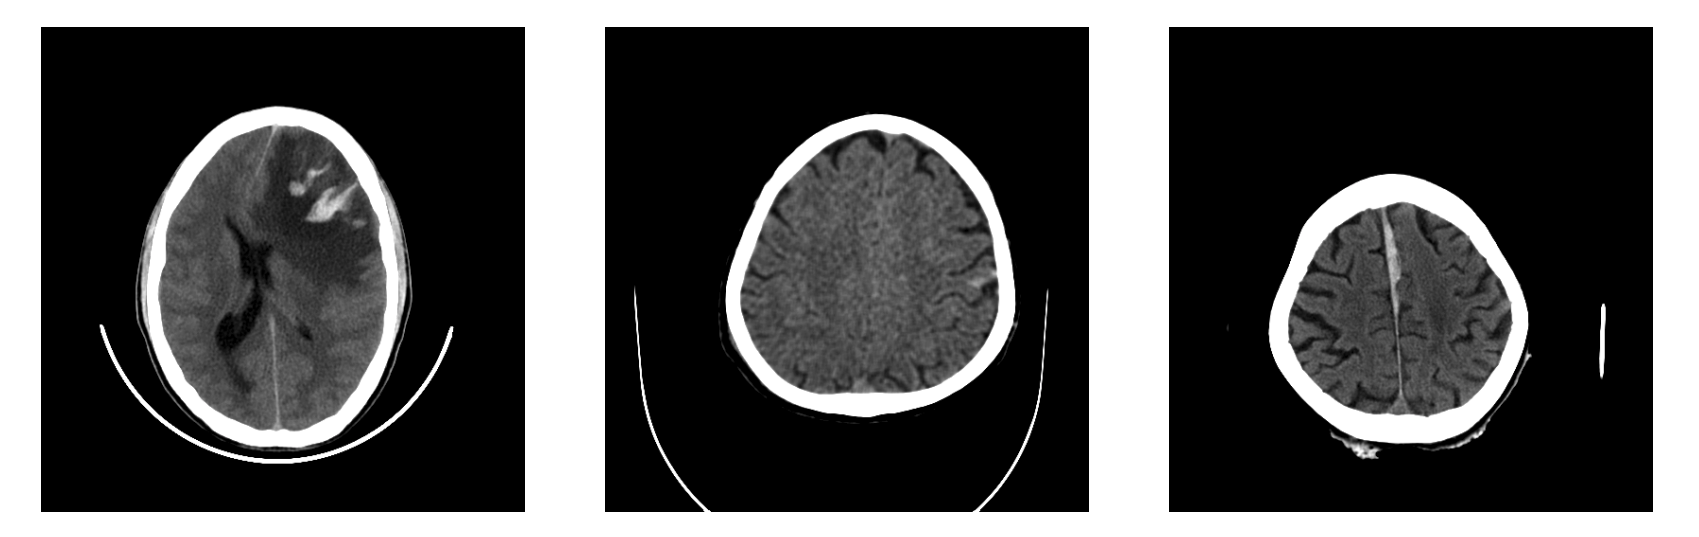
\includegraphics[width=1\columnwidth]{02-related-works/figures/sample-ct-images.png}}
    \caption{Sample CT Images \cite{chilamkurthy2018deep}}
    \label{fig:sample-ct-images}
\end{figure}

                    Analyzing the parts of human body, diagnosing the abnormalities and traumas, observing the results of the cancer treatments are the common use cases of CTs.
                    It comes with several benefits sucs as getting good spatial resolution, detecting issues quickly and painlessly.
                    On the other hand, CTs do not provide real time analysis and relatively useless results with the soft tissues with low contrast.

                %! Author = fatihergin
%! Date = 2020-05-03

\begin{table}[h]
\caption{Comparision of medical imaging techniques}
\centering
\begin{tabular}{c|cccc}
Imaging Techniques         & \begin{tabular}[c]{@{}c@{}}Spatial \\ resolution\end{tabular} & \begin{tabular}[c]{@{}c@{}}Good \\ contrast\end{tabular}          & Cost   & \begin{tabular}[c]{@{}c@{}}Real time \\ visualization\end{tabular} \\
\specialrule{2pt}{1pt}{1pt}
Ultrasonography            & 1mm                                                          & Soft tissues                                                      & Low    & Supported                                                           \\
X-ray                      & 1mm                                                          & \begin{tabular}[c]{@{}c@{}}Soft tissues \\ and fluid\end{tabular} & Medium & Unsupported                                                        \\
CT                         & 0.5mm                                                        & \begin{tabular}[c]{@{}c@{}}Hard and \\ soft tissues\end{tabular}  & High   & Unsupported                                                         \\
MRI                        & 0.5mm                                                        & \begin{tabular}[c]{@{}c@{}}Hard and \\ soft tissues\end{tabular}  & High   & Unsupported                                                         \\
\hline
\end{tabular}
\label{table:comparision-of-medical-imaging-techniques}
\end{table}

        \end{itemize}

        A general comparison for common medical imaging technique is given in Table ~\ref{table:comparision-of-medical-imaging-techniques}.
        Ultrasonography which is the first technique in Table ~\ref{table:comparision-of-medical-imaging-techniques} is examined in Section ~\ref{subsection:dermatology-imaging-techniques}.

    \subsection{Dermatology Imaging Techniques} \label{subsection:dermatology-imaging-techniques}

        In this section, imaging techniques used in skin lesions are being investigated.

        \begin{itemize}

            \item \textbf{Traditional Photography (TP)} is the well-known techniques which makes visualizing and monitoring the top layer of the lesion possible \cite{feit2004melanomas}.

            \item \textbf{Dermoscopy Imaging Technique (DIT)} is a real-time noninvasive diagnostic imaging technique
                    which is more successful in distinguishing melanoma concentration than traditional photography \cite{aljanabi2019various}.

            \item \textbf{Multispectral Imaging (MI)} provides information in both spectral and spatial domains.
                    MI systems increase accuracy by calibrating image intensity,
                    controlling exposure time automatically with the help of a multispectral camera that includes different optical filters selected by the problem definition.
                    MI is used in medical imaging to support  detecting the lesions about 2 mm \cite{aljanabi2019various}.
                    Figure~\ref{figure:sample-multispectral-images} shows the images of a skin lesion taken by using different optical filters.

                    \begin{figure}
    \centerline{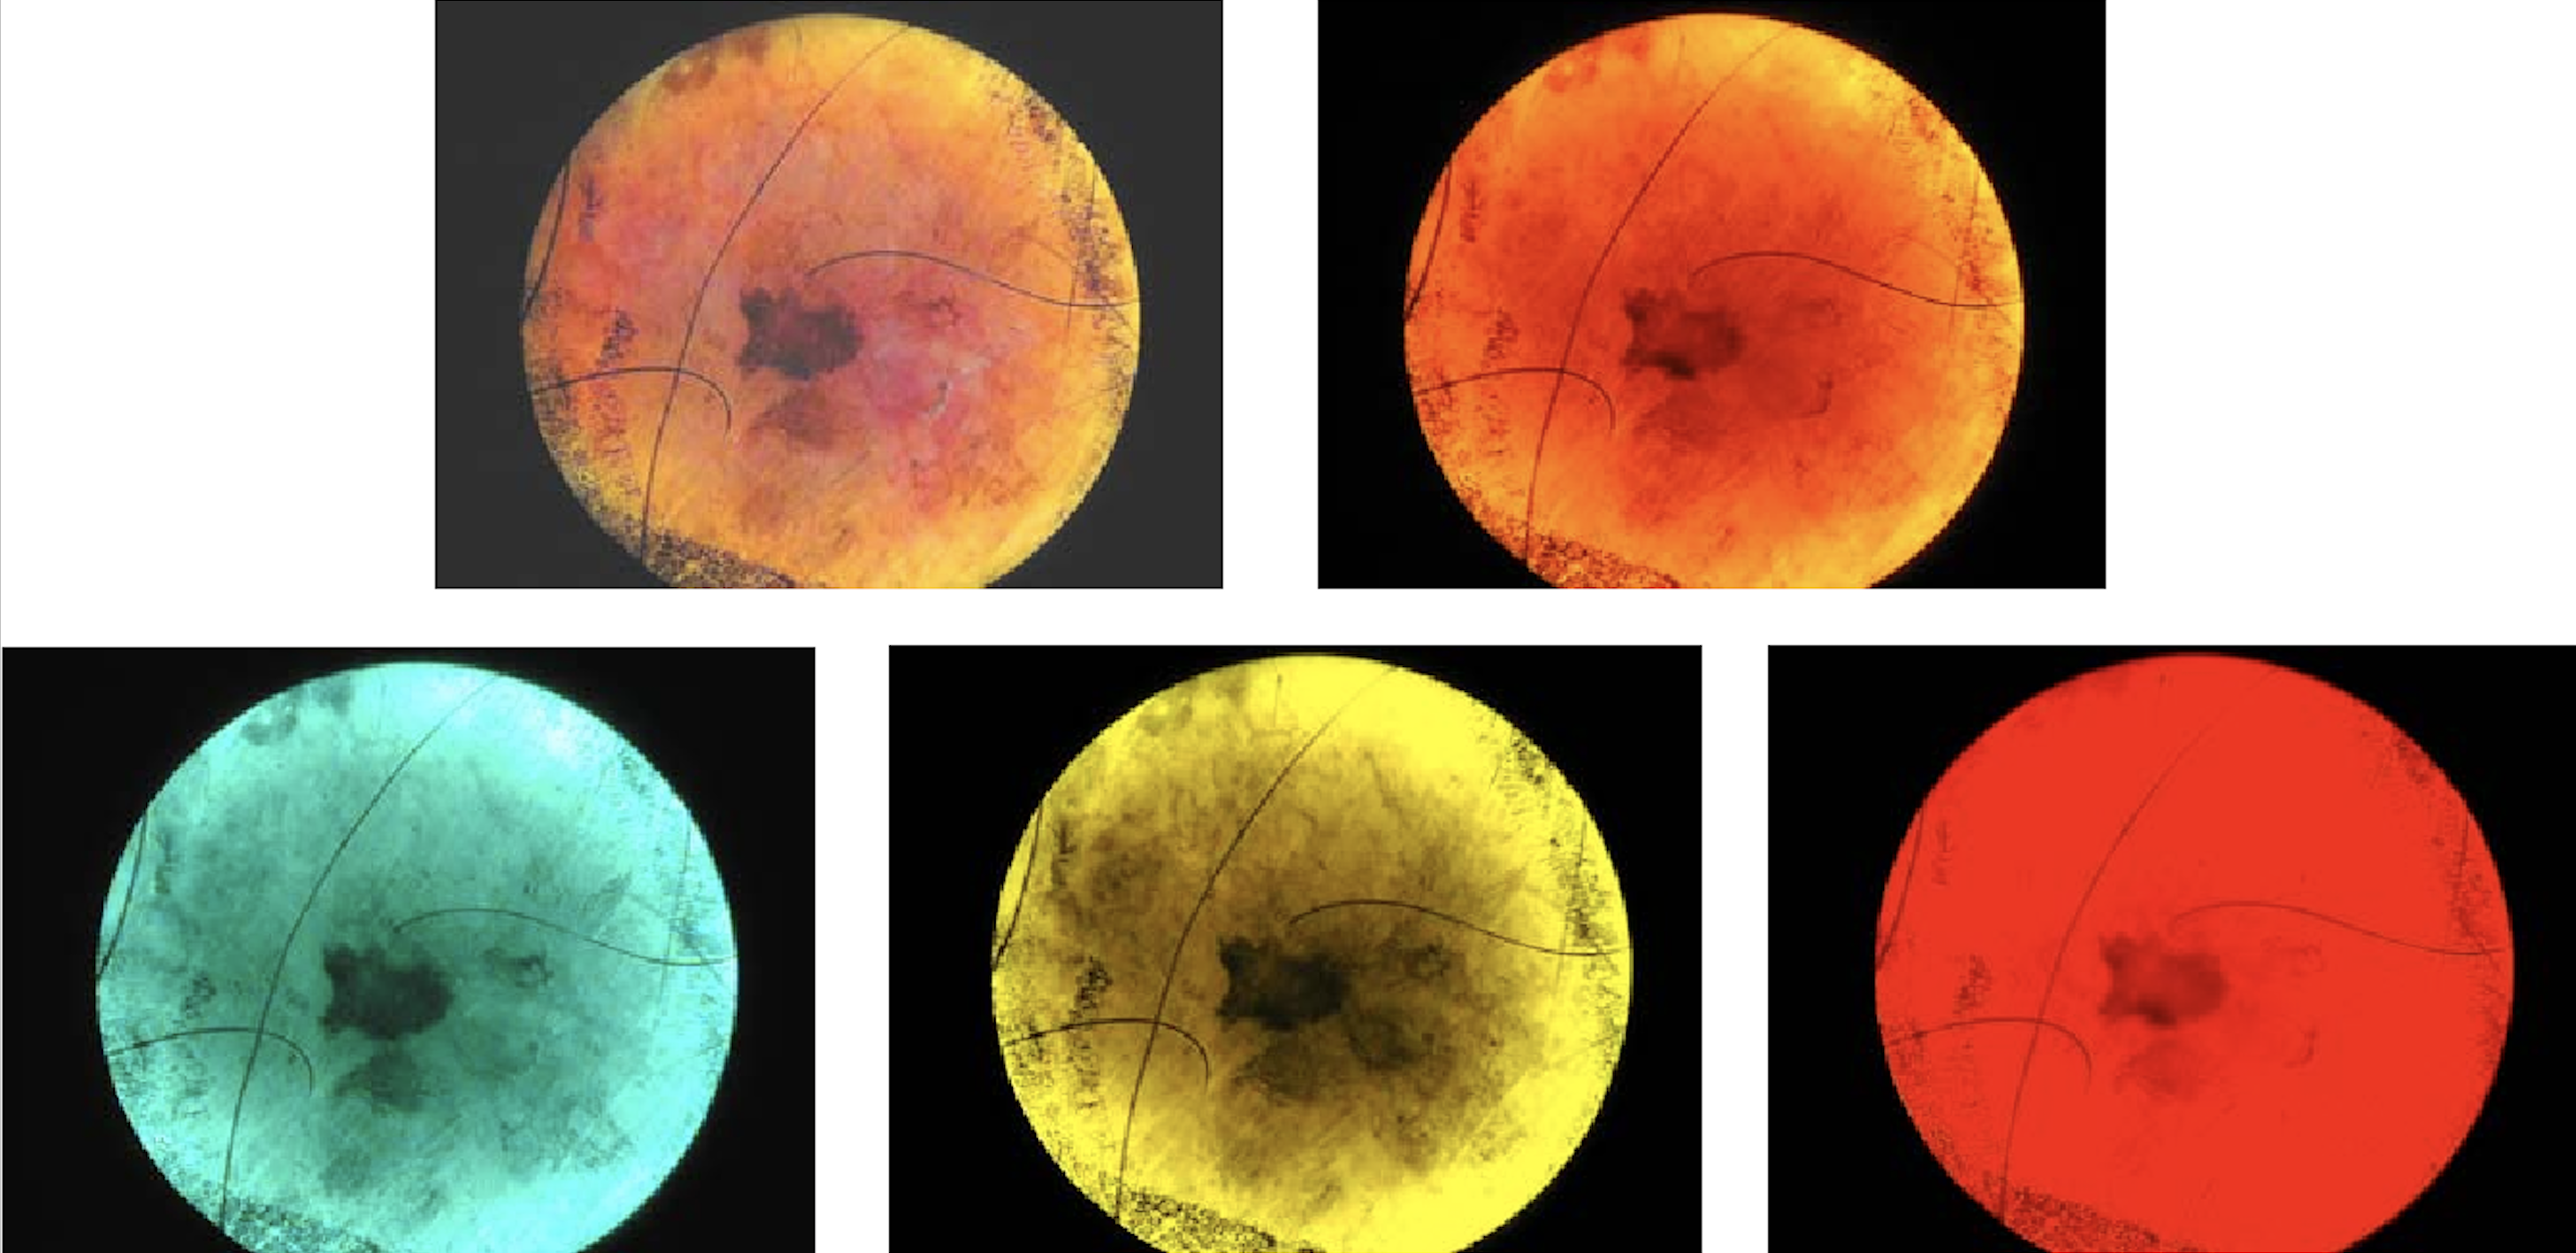
\includegraphics[width=1\columnwidth]{02-related-works/figures/sample-multispectral-images.png}}
    \caption{Sample Multispectral Images \cite{dhawan2009multispectral}}
    \label{figure:sample-multispectral-images}
\end{figure}

            \item \textbf{Confocal Laser Scanning Microscopy (CLSM)} is an imaging technique that provides real-time details of skin morphology
                    and provides images with the same resolution as traditional microscopes \cite{gerger2005diagnostic}.
                    CLSMs are very sensitive for clinical applications but they are relatively expensive to use in there.
                    From right to left clinical, dermoscopical, confocal images of a skin lesion is shown in Figure~\ref{figure:sample-clsm-images}.

                    \begin{figure}
    \centerline{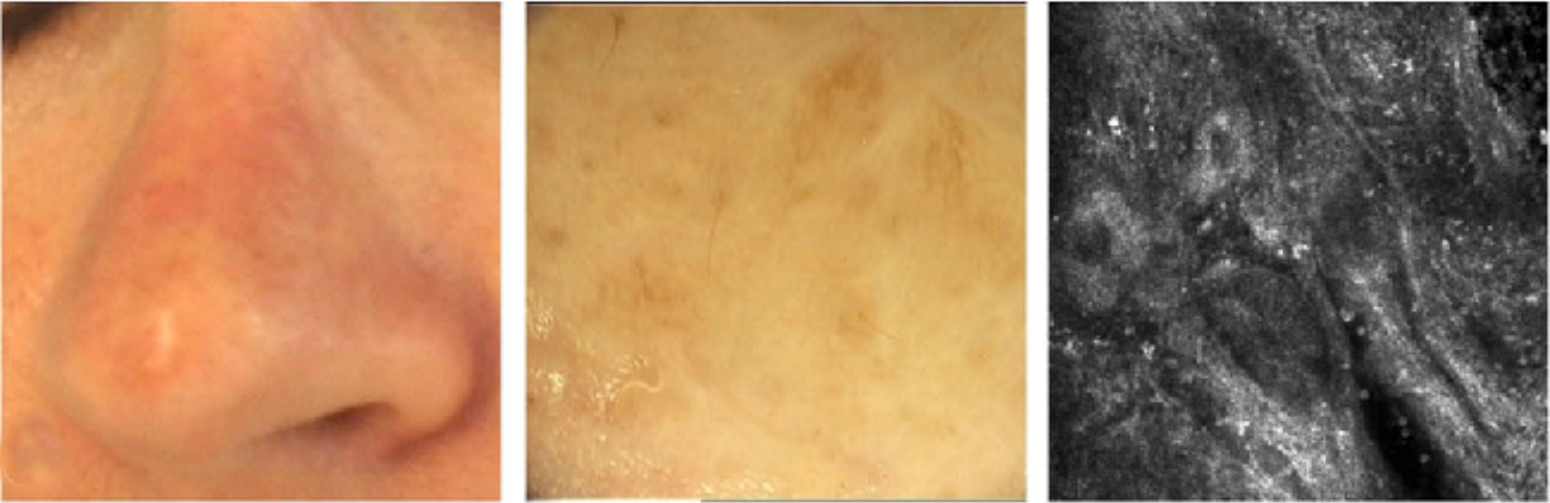
\includegraphics[width=1\columnwidth]{02-related-works/figures/sample-clsm-images.png}}
    \caption{From right to left clinical, dermoscopical, confocal images of a skin lesion \cite{ruini2016invisible}}
    \label{figure:sample-clsm-images}
\end{figure}

            \item \textbf{Ultrasonography} which is also known as diagnostic sonography is another imaging technique that is used to create medical imaging to create internal body parts using high frequency broadband sound waves.
                    Because different tissues behave differently under these sound waves,  the images generated using the waves reflected by tissue \cite{sahuquillo2013study}.
                    Calculating the depth of skin cancer is the focused usage of Ultrasonography for this kind of projects.

                    Ultrasonography offer painless real time visualization without ionized radiation in high resolution.
                    But it is a time consuming and operator dependendent imaging technique.

        \end{itemize}
